\begin{frame}{finding objects}
    \begin{itemize}
    \item most simple approach:
        \begin{itemize}
        \item everyone sent full list of nodes and their IP/port/etc.
        \item works for small DHT-like design
        \item example: DynamoDB (in-datacenter database)
        \end{itemize}
    \item simple distributed approach:
        \begin{itemize}
        \item everyone has successor node
        \item go around the ring until you find the right node
        \end{itemize}
    \end{itemize}
\end{frame}


\begin{frame}{shortcuts}
    \begin{itemize}
    \item problem with simple approach: N steps
    \item optimization:
        \begin{itemize}
        \item if we know a few other nodes\ldots
        \item can start at one that's closer
        \end{itemize}
    \item question: which other nodes to know
    \end{itemize}
\end{frame}

\begin{frame}{finger tables}
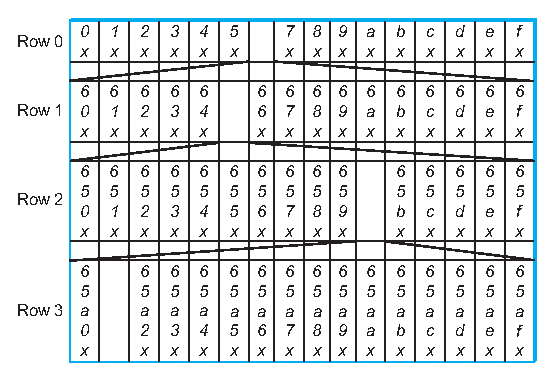
\includegraphics[width=\textwidth]{../p2p/sysapp-fig242}
\end{frame}

\begin{frame}{finger table idea}
    \begin{itemize}
    \item if my ID is 0x65a1fc\ldots
    \item track something like
        \begin{itemize}
        \item node for 0x0000\ldots, 0x1000\ldots, 0x2000\ldots, \ldots
        \item node for 0x6000\ldots, 0x6100\ldots, 0x6200\ldots, \ldots
        \item node for 0x6500\ldots, 0x6510\ldots, 0x6520\ldots, \ldots
        \item node for 0x6510\ldots, 0x6511\ldots, 0x6512\ldots, \ldots
        \item \lots
        \end{itemize}
    \item (not the only possible choice)
    \end{itemize}
\end{frame}

\begin{frame}{DHT variations}
    \begin{itemize}
    \item different notion of `closest' 
        \begin{itemize}
        \item next hash value with wraparound not only option
        \end{itemize}
    \item different ideas of how to manage finger tables
    \end{itemize}
\end{frame}
